\section{Durchführung}
\label{sec:Durchführung}
\subsection{Aufbau}
\begin{figure}[H]
  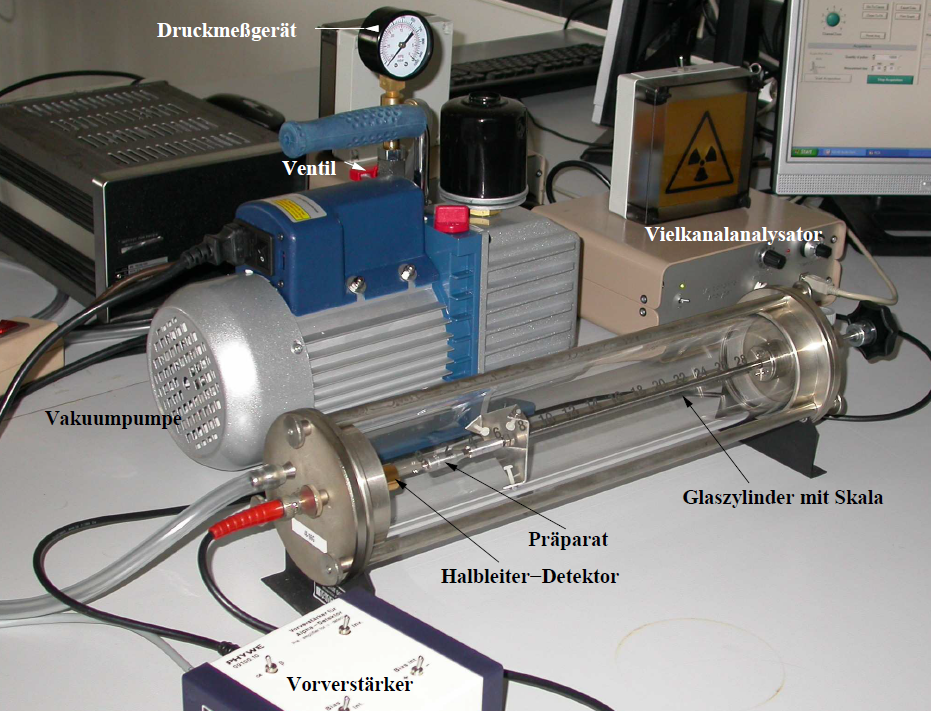
\includegraphics[scale=0.6]{Text/Bilder/Aufbau.PNG}
  \caption{Aufbau zur Bestimmung der Reichweite von $\alpha$-Strahlung\cite[3]{sample}}
  \label{fig:Aufbau}
\end{figure}
\noindent
Der in Abbildung \ref{fig:Aufbau} zu sehende Aufbau besteht aus einem Glaszylinder, in dem sich ein Halbleiter-Detektor und das Am-Präparat befinden, einer Vakuumpumpe sowie
einem Vorverstärker und einem Vielkanalanalysator. Die einzelnen Komponenten werden gemäß Abbildung \ref{fig:Aufbau} verbunden und wird für die im folgendem
erläuterten Versuchsteile verwendet.

\subsection{Bestimmung der Reichweite von Alpha-Strahlung}
Zunächst wird der Glaszylinder evakuiert, sodass ein Druck von ungefähr $\SI{0}{\milli \bar} $ herrscht. Der Abstand zwischen Präparat und
Halbleiter-Detektor wird auf $\SI{23}{\milli \meter}$ eingestellt. Die Zählraten $N$ werden bei einer Messzeit von $\Delta t=\SI{120}{\second}$ gemessen und der Druck in
$\SI{50e-3}{\bar}$-Schritten erhöht.
Dies wird für einen Abstand von $\SI{24}{\milli \meter}$ wiederholt.

\subsection{Statistik des radioaktiven Zerfalls}
Der Abstand zwischen Präperat und Halbleiter-Detektor wird auf $\SI{20,5}{\cm}$ eingestellt.
Der Glaszylinder wird evakuiert und die Zählrate $N$ in einem Zeitintervall von $\SI{10}{\second}$ 100 mal gemessen.
